%
% File acl2016.tex
%
%% Based on the style files for ACL-2015, with some improvements
%%  taken from the NAACL-2016 style
%% Based on the style files for ACL-2014, which were, in turn,
%% Based on the style files for ACL-2013, which were, in turn,
%% Based on the style files for ACL-2012, which were, in turn,
%% based on the style files for ACL-2011, which were, in turn, 
%% based on the style files for ACL-2010, which were, in turn, 
%% based on the style files for ACL-IJCNLP-2009, which were, in turn,
%% based on the style files for EACL-2009 and IJCNLP-2008...

%% Based on the style files for EACL 2006 by 
%%e.agirre@ehu.es or Sergi.Balari@uab.es
%% and that of ACL 08 by Joakim Nivre and Noah Smith

\documentclass[hidelinks, 11pt]{article}
% for table colouring 
% \usepackage[table]{xcolor}
\usepackage[table]{xcolor}
\usepackage{acl2016}
\usepackage{times}
\usepackage{url}
\usepackage{latexsym}

% for todo notes 
\usepackage{todonotes}

% maths
\usepackage{amssymb}
% cool maths printing
\usepackage{amsmath}

\usepackage[hidelinks]{hyperref}
% For referencing sections across the article
\usepackage{cleveref}

\aclfinalcopy % Uncomment this line for the final submission
%\def\aclpaperid{***} %  Enter the acl Paper ID here

%\setlength\titlebox{5cm}
% You can expand the titlebox if you need extra space
% to show all the authors. Please do not make the titlebox
% smaller than 5cm (the original size); we will check this
% in the camera-ready version and ask you to change it back.

\newcommand\BibTeX{B{\sc ib}\TeX}
% To add some line spacing in the table
\renewcommand{\arraystretch}{1.3}

\title{Detecting agreement in a multi-party conversation}

\author{Tom Byars, Cale Clark, Charlie Lyttle, Katie McAskill, Jack Miller, Zein Said, \\
{\bf Laura Schauer, Jason Sweeney, Aron Szeles, Xander Wickham} \\
School of Mathematics and Computer Science, Heriot-Watt University, Edinburgh \\ {\tt {[tjb10, cc164, cl157, klm12, jjm7, zs2008,}} \\ {\tt {lms9, js418, as472, aw127]}@hw.ac.uk}}

\date{February 2023}

\begin{document}
\maketitle

\begin{abstract}
  Today, conversational systems are expected to handle conversations in multi-party settings. However, practical usability remains difficult as there are additional challenges to overcome, such as speaker and addressee recognition and turn-taking. In this paper, we present our work on a multi-party conversational system, which invites two users to play a trivia game in a hospital waiting area. The system detects users' agreement or disagreement on a final answer and responds accordingly. Our evaluation includes both performance and user assessment results, and we have configured the system to be used on the ARI robot deployed in a hospital waiting area as part of the SPRING project.
\end{abstract}


\section{Introduction}
\label{sec:introduction}

Socially assistive robots (SARs) are a crucial part of the future of many sectors, for example, education or healthcare \cite{gunson_visually_aware_2022}. Especially the latter depends on technology advancements as it is facing numerous obstacles in the future, such as increasing spendings and a growing percentage of older people. A serious lack of healthcare workers is already being experienced, with 10 million more health workers needed worldwide by 2030 \cite{cooper_ari_2020,Health_workforce_2023}. SARs can pose a solution to the problem by supporting healthcare in various ways, such as encouraging older people to keep living independently longer or reducing caregiver burden \cite{cooper_ari_2020}.

Healthcare SAR scenarios frequently require SARs to handle multi-party interactions as it is likely in these situations that more than one person will interact with the system (i.e., a hospital waiting room). Therefore, we propose a conversational system in this work that plays a game of ``Who wants to be millionaire?'' with two people. Our system impersonates the host while participants can collaborate on general knowledge trivia questions.

The conversational system is trained on multi-party human-human conversation data. We collected the data from recordings of special “Who wants to be millionaire?“ episodes where two candidates collaborated to answer the host's questions.

Our system is developed to be fitted onto an ARI robot in the course of the SPRING-ARI project. This project encompasses several European universities collaborating on evolving socially assistive robots. They use an ARI robot, which is deployed in a hospital waiting area in France.

\section{Background}
\label{sec:background}

\subsection{Socially Assistive Robots}
\label{subsec:socially_assistive_robots}
For healthcare, as well as for any other sector, the difficulty of successfully designing SARs lies in creating robots that can effectively converse with humans and adhere to social norms \cite{moujahid_multi_party_2022}. The more expressive a robot is, the more it will be perceived as intelligent, conscious and polite \cite{moujahid_multi_party_2022}.

The SPRING project conducts research on a SAR robot deployed in an eldercare hospital reception area \cite{addlesee_comprehensive_2020}. The conversational system is deployed on the humanoid ARI robot produced by Pal Robotics \cite{palrobot}. ARIs capabilities can be extended with custom AI algorithms, in the case of SPRING-ARI a visual perception system, a dialogue system, and a social interaction planner \cite{addlesee_comprehensive_2020}. While the SPRING-ARI system successfully demonstrates that task-based, social and visually grounded dialogue can be combined with physical actions, it still lacks the ability to handle conversations with more than one person simultaneously \cite{addlesee_comprehensive_2020}.

\subsection{Multi-party Human Robot Interaction}
\label{subsec:multi_party}
The endeavour to create conversational systems becomes considerably more difficult when dealing with multi-party interactions \cite{Addlesee_Data_2023}. Compared to handling dyadic (two-party) interactions, handling multi-party conversations includes more complex challenges, such as Speaker Recognition, Addressee Recognition, Response Selection (summarised in “who says what to whom“) and coordination of turn-taking \cite{Addlesee_Data_2023,Johansson_Skantze_2015}.

Especially turn-taking poses a central problem. It is defined as follows:

\begin{quote}
  The rules of turn-taking organize the conversation into turns, during which one of the participants has the right to speak while the others agree to listen. \cite{Żarkowski_2019}
\end{quote}

In dyadic conversations, there are only two roles a participant can take: speaker or listener, hence it is clear when and to whom the turn is yielded. In multi-party conversations, participants can take multiple roles, therefore turn-taking needs to be coordinated \cite{Johansson_Skantze_2015}. Humans signal their intents mostly through gaze, but also through pauses, prosody, and body positioning \cite{Żarkowski_2019}. To copy this behaviour, earlier models for conversational systems relied on silence time-outs to coordinate turn-taking, however, this approach is found to be too simplistic \cite{skantze_turn_taking_2021}. Instead, mimicking human turn-taking behaviour better by using a combination of verbal and non-verbal cues leads to robots that are better perceived \cite{moujahid_multi_party_2022}.




\section{Data Collection}
\label{sec:data_collection}

An important point to consider in multi-party training data is that most are human-human. This can pose a problem as systems trained on human-human conversations may lack the incentive to help users reach their goals \cite{Addlesee_Data_2023}. This is not true for our scenario, as our system's goal is to imitate the host of the game show ``Who wants to be millionaire?''. In this game, the host has the clear goal of guiding the participants to finding an answer to a question. However, to our knowledge, there are no multi-party corpora available for this use case, therefore data collection was performed by our team. We first collected all available recordings of ``Who Wants to Be a Millionaire'' with two participants, which were transcribed using the YouTube API. To annotate these transcripts, we used the set of annotations shown in \Cref{table:intents}. This list allows us to capture as much information as possible, without saturating the data.

\noindent
\begin{table}[h!]
  \begin{tabular}{ | p{2cm} | p{5cm} | }
    \hline
    \rowcolor[HTML]{BFD8EC}
    \textbf{Intent}      & \textbf{Description}                                                     \\
    \hline \hline
    \rowcolor[HTML]{DCE9F6}
    \multicolumn{2}{|c|}{\textit{Host (System) Intents}}                                            \\
    \hline
    question             & The system presents the question                                         \\
    \hline
    options              & The system presents the options                                          \\
    \hline
    confirm-agreement    & The system tries to confirm the final answer with participants           \\
    \hline
    accept-answer        & System considers answer the final answer                                 \\
    \hline \hline
    \rowcolor[HTML]{DCE9F6}
    \multicolumn{2}{|c|}{\textit{User Intents}}                                                     \\
    \hline
    chit-chat            & Speech not related to the quiz                                           \\
    \hline
    offer-answer()       & A player presents an answer to the other player                          \\
    \hline
    offer-to-answer      & A  player signals that they know the answer                              \\
    \hline
    agreement            & Agreement between players about the answer                               \\
    \hline
    ask-agreement        & A player asks the other player for confirmation on their proposed answer \\
    \hline
    final-answer()       & Players give final answer                                                \\
    \hline
    confirm-final-answer & Participants confirm their answer is final                               \\
    \hline
  \end{tabular}
  \caption{Intents used for Data Annotation}
  \label{table:intents}
\end{table}

\subsection{Cohen's Kappa Coefficient}
To ensure reliability and consistency, Cohen's kappa was calculated for a sample of the completed transcripts. It measures the reliability between raters on categorical data, while accounting for agreement happening by chance \cite{Cohen_1960}. A sample of four transcripts are re-annotated by a team member, which amounts to approximately 15\% of the total transcripts.

\begin{equation}
  \begin{split}
    KappaScore & = \frac{Agree - ChanceAgree}{1 - ChanceAgree} \\
    KappaScore & = \underline{\underline{0.9601}}
  \end{split}
\end{equation}

\noindent
A Kappa score of 0.9601 is interpreted as ``almost perfect agreement'' \cite{McHugh_2012}. From this, the annotation of transcripts can be concluded as reliable.


% DESIGN & IMPLEMENTATION
\section{Design and Implementation}
\label{sec:implementation}

Our conversational system consists of several parts, the modular architecture is shown in \Cref{fig:system_architecture}. This section outlines each unit and describes how our system manages the process from the users' utterances to selecting its response.

\begin{figure*}
  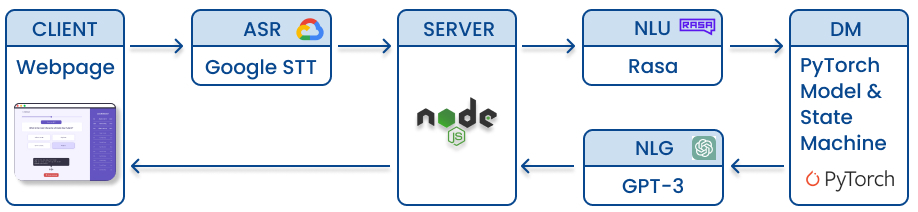
\includegraphics[width=\textwidth]{images/sys_graph.jpg}
  \caption{Architecture of the conversational system}
  \label{fig:system_architecture}
\end{figure*}

\subsection{Automatic Speech Recognition}
\label{subsec:asr}

The first step is to transform user's speech into text, which can be passed onto Natural Language Understanding (NLU) to perform intent recognition. Transforming audio into text works through Speech-To-Text (STT) software. In recent years, STT systems have become more accurate and fast, however, none of the existing systems can yet reliably handle conversations in real-time \cite{addlesee_comprehensive_2020}.

Our conversational system required two non-standard features from the ASR: (1) real-time transcription and (2) diarization. Given that our system was designed for usage on a robot, it must transcribe what the user is saying in real-time to avoid response delays and ensure natural sounding conversation. Therefore, the time taken for a system to respond can only be marginally longer than the delay a human would leave before responding \cite{Miller_1968}.

The second feature, diarization, is the process of determining the speaker in multi-party conversations. To handle a ``Who wants to be millionaire?'' style game, our system must be able to diarise to track the intents of each individual user and determine when users agree or disagree. We tried several STT systems including Amazon's Transcribe, IBM's Watson and locally running Pyannote. Our findings were that these are all suitable for transcription but lack real-time diarization. We settled with Google's Cloud Speech-to-Text API due to its high accuracy and customisability. As it is widely used, troubleshooting and integration resources were readily available. In addition, Google's API promised diarization capabilities, which, along with its real-time transcription capabilities seemed to fit our use case. However, in use, diarization was inaccurate, and it often grouped two separate speakers together or split sentences up seemingly at random. This became even more apparent when two users were speaking over each other, supporting the statement that ASR systems are not yet adequate to reliably handle natural spontaneous conversations in real-time \cite{addlesee_comprehensive_2020}.

This made Google's diarization unusable for our use case. We therefore moved to a set-up with two microphones (one for each user) and integrated them with the real time Google transcription. By removing diarization we were able to use the most up-to-date Google model \verb|latest_long|, which is trained on long-form conversation. This allowed us to not only avoid the issue of diarization, but also to improve the quality of the transcriptions, which had a cascading effect on the rest of the system, leading to better intent recognition, entity extraction, etc.

A drawback of this set-up is that the microphones may pick up both user's voices. This could be mitigated through moving the microphones further apart, or calibrating them. More on this issue is discussed in \Cref{sec:evaluation}.

The real-time transcription of the users' utterances are then passed onto NLU.

\subsection{Natural Language Understanding}
\label{subsec:nlu}

Natural Language Understanding takes in utterances of natural human language and classifies them into intents. RASA is an open-source framework for building conversational systems, which offers NLU tools. We used its NLU tool to train on our pre-processed data. RASA NLU successfully created a model that can accurately label new, unseen inputs from the ``Who wants to be millionnaire'' game domain with an intent from the list given in \Cref{table:intents}.

The model is also capable of entity extraction, which means it can identify words of interest. In our case, we extract a user's answer to a question or a user's rejected answer given from an utterance. For example, a user's utterance could be ``I'm thinking Teaspoon'', which would be classified by the NLU in the following way:

\begin{verbatim}
NLU:    - intent: offer-answer
          entities:
            - answer: "Teaspoon"
\end{verbatim}

\subsubsection{Evaluation of NLU}
\label{subsec:NLU_evaluation}

An initial model trained on only four annotated transcripts, very little training data was highly innacurate, mislabelled intents, and extracted wrong answers or no answer at all. The accuracy for this model was 47\% with a macro-averaged F1-Score of 0.43.

Using a larger volume of training data significantly improved NLU performance. The model used in our system was trained on 25 transcripts with 566 training examples for each intent. Additional improvement could be obtained by manually cleaning the training data of any misplaced or wrongly extracted examples.

As can be seen in \Cref{fig:cm_answer_extraction}, the improved model's confusion matrix is perfect. \Cref{fig:cm_intent_recognition} shows the intent confusion matrix. This model has an accuracy of 96.3\% with a macro-averaged F1-Score of 0.96.

The intents identified by the NLU are then passed onto the DM unit.

\begin{figure}[h!]
  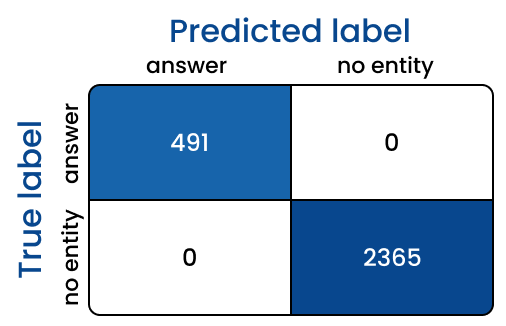
\includegraphics[width=\columnwidth]{images/answer_confusion_matrix.jpg}
  \caption{Confusion Matrix of NLU answer extraction}
  \label{fig:cm_answer_extraction}
\end{figure}

\begin{figure}[h!]
  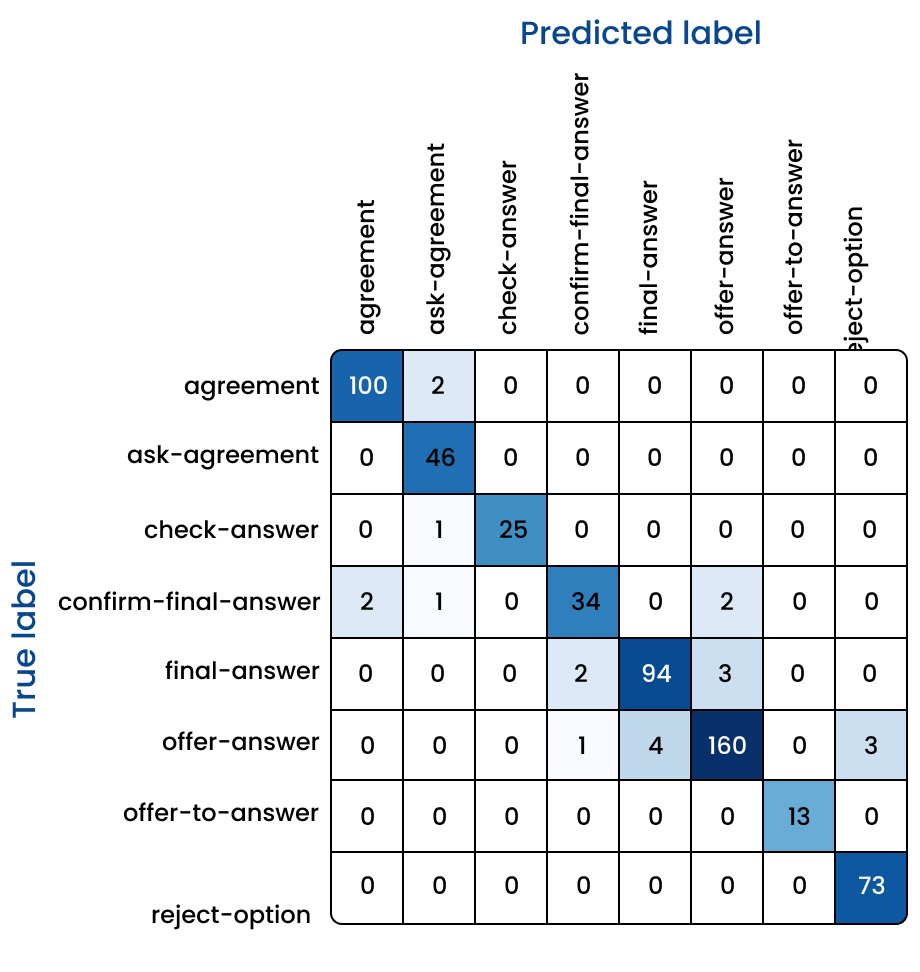
\includegraphics[width=\columnwidth]{images/intent_confusion_matrix.jpg}
  \caption{Confusion Matrix of NLU intent recognition}
  \label{fig:cm_intent_recognition}
\end{figure}

\subsection{Dialogue Management}
\label{subsec:dialogue_management}

The dialogue manager is composed of two components: a state machine and a Pytorch model. This approach was chosen because, despite involving a conversation which requires intelligent behaviour from the dialogue manager, the game itself is defined by a set of rigid rules:
\begin{itemize}
  \item The users are always asked ten questions.
  \item The system must drive the conversation by passing from one question to the next.
  \item The game must end at a specified time.
\end{itemize}
\noindent Occasionally overwriting the model's output with the hard-coded logic of the state machine ensure these rules are followed and that the movement from state to state is observed.

\subsubsection{Neural Network}
\label{subsec:nn}
The neural network model is needed to be designed to manage dialogues of three-person conversations. To do this, it has two inputs, the intent from the NLU and the user ID (user 1, user 2 or host). These inputs were both one-hot encoded, the intent being a vector of size 14 (one for each intent) and the user number being a vector of size 3. These two vectors were concatenated to produce an input vector of size 17. The network was then trained to predict the host's response for a given intent and user in a sequence. This output is a vector of size 5, one for each of the 4 system intents plus one for \verb|no response| (see \Cref{table:intents}).

The model was trained using the dataset which we had originally labelled for NLU purposes. This provided human labelled sequences of intents and user IDs for each question. Each question would have its intents and user IDs input into the network sequentially, with the model's memory being cleared after every question. Every output from the system which is not \verb|no response| would be input back into the network, allowing for the system to speak multiple lines of dialogue in succession. At the start of each question, the system is set up by first inputting the host having given the \verb|question| intent, to which it will always output the \verb|options| intent. This is required since every question in the training data is started by the host asking the question, then giving the options for the question.

The primary difficulty of training was the imbalance in the dataset. Since most of the time, the host will be only listening, \verb|no response| is by far the most common output. This means that having the output as a single SoftMax vector of size 5 would be difficult, as the model would quickly learn to always output \verb|no response|. Traditional undersampling and oversampling methods would also be difficult to make use of, since the \verb|no response| output exists as part of a real conversation, which must be fed into the network sequentially. For example, uncommon system responses could not be oversampled, as they exist as part of a real question, most of which is often filled with \verb|no response| from the host. Artificially increasing their frequency could not be done without altering the questions, which would diminish the integrity of the data.

\begin{figure}
  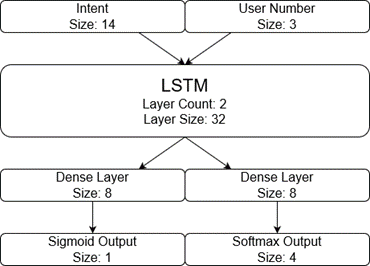
\includegraphics[width=\columnwidth]{images/DM_LSTM.png}
  \caption{Architecture of PyTorch Model}
  \label{fig:model_architecture}
\end{figure}

To overcome this, a separate Sigmoid output was used for \verb|no response|, as shown in \cref{fig:model_architecture}. To train this model, whenever \verb|no response| from the host was expected, the loss from the SoftMax vector was set to zero, otherwise L2 loss was used for all outputs. The system was implemented in PyTorch, with the model being trained for 30 epochs with a learning rate of 5x10-4.

In future, this architecture could be used for handling multi-person dialogues with more intents or more users by simply scaling the inputs, outputs, and hidden layers accordingly. The model could also be altered to allow for more inputs such as pauses or other non-verbal cues.

\paragraph{Neural Network Architectures}
\label{par:nn_architectures}

\begin{itemize}
  \item difference between LSTM \& RNN
  \item why not RASA, but own DM
\end{itemize}

\subsubsection{Dialogue Manager - Jack}
\label{subsec:dm}

An intent received from the NLU unit is first input into the PyTorch model. The model then decides on an appropriate action. Afterwards, the state machine checks if the output of the PyTorch model represents a sensible action. In case there are logical errors, the output will be overridden. For example, if the NLU detects that the user intends to confirm their final answer, but no answer has yet been given, the PyTorch model may nonetheless decide on \verb|accept-answer|. As no answer has been given yet, the state machine will overwrite this output.

Another reason for using a state machine was the limited amount of transcription data. The PyTorch model learned off of the transcript data, therefore it depended on a sufficient amount of transcript data to function adequately. Using a state machine allowed us to program explicitly how the chatbot responds to user intents, thus eliminating the need for more transcript data.

\begin{figure}[h!]
  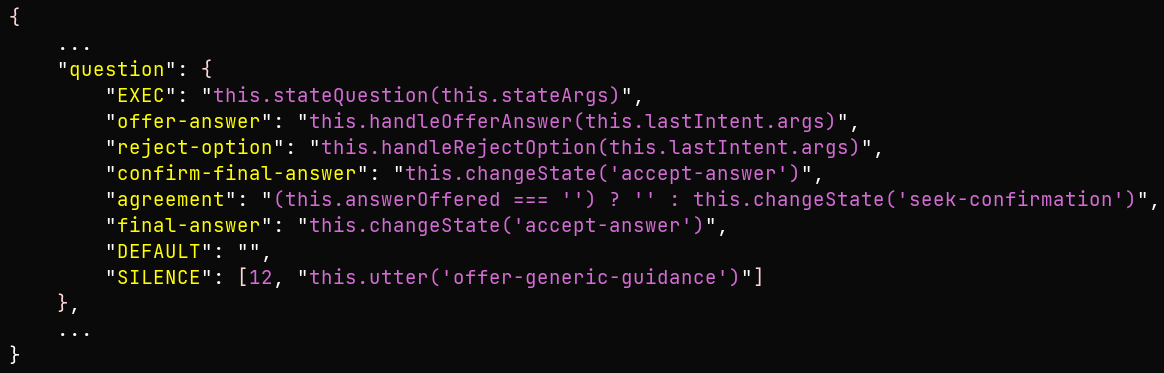
\includegraphics[width=\columnwidth]{images/jacks_figure.png}
  \caption{State Machine behaviour}
  \label{fig:jacks_figure}
\end{figure}

The state machine's configuration is defined inside a JSON file, as shown in \Cref{fig:jacks_figure}. The figure shows the behaviour of the state machine when the state is \verb|question|. An example of previously recorded values influencing the flow can be seen inside \verb|agreement|. When the action decided by the chatbot is overridden by the state machine, it is done according to this configuration. The action chosen by the state machine is a string of JavaScript code, and is found in the configuration object \verb|flow| at \verb|flow[state][intent]|, where \verb|state| is the current state of the machine and \verb|intent| is the name of the most recent user intent.

Throughout the course of a game, the dialogue manager stores relevant values, such as answers offered by the user. These values influence the behaviour of the state machine. An example of this can be observed inside the \verb|seek-confirmation| state when the host asks if the user would like to lock in an answer suggested by them. If a user declines, the host checks if the rejected answer is the same as the one just offered by the user. If it matches, then the host assumes that the user does not want to lock in that answer. However, if the answer rejected by the user is another one, then the host will assume that they do indeed wish to proceed with their offered answer.

\noindent
\begin{table}[h!]
  \begin{tabular}{ | p{2cm} | p{5cm} | }
    \hline
    \rowcolor[HTML]{BFD8EC}
    \textbf{Intent}           & \textbf{Description}                                                                                                                      \\
    \hline
    acknowledge-reject-option & The system acknowledges that a player has dismissed an option and may ask them for a reason.                                              \\
    \hline

    end-of-game               & The system announces the end of the game and informs the players of how they did.                                                         \\
    \hline

    offer-generic-guidance    & The system offers advice or encouragement to the players.                                                                                 \\
    \hline

    question-brief            & The system restates the current question number and question prize.                                                                       \\
    \hline

    repeat-answer             & The system repeats a player's answer back to them.                                                                                        \\
    \hline

    return-to-question        & The system returns to the question state, becoming less insistent on locking in answers suggested.                                        \\
    \hline

    say-correct               & The system states that the players's final answer was correct.                                                                            \\
    \hline

    say-incorrect             & The system states that the players's final answer was incorrect.                                                                          \\
    \hline

    seek-confirmation         & The system asks the players if they are wishing to lock in a suggested answer as final.                                                   \\
    \hline

    seek-direct-answer        & The system asks the players to state their answer. This is done by the system when it suspects that it may have missed an answer offered. \\
    \hline
  \end{tabular}
  \caption{Additional State Machine Intents}
  \label{table:state_machine_intents}
\end{table}
A more secure approach to this situation would involve taking a record of all the answers ruled out by the users. The host would then lock in a final answer after a rejected answer if and only if the other two possible answers had also been previously rejected. We would take in a future implementation as it would reduce the risk of the host accepting answers while the users are still deciding.

\subsection{Natural Language Generation}
\label{subsec:nlg}

To make the system feel more unique and less robotic, we made use of Natural Language Generation (NLG) for the phrases that the “host” says to the participants. We used OpenAI's API, specifically “gpt-3.5-turbo”, the same version that is used in ChatGPT. This allowed us to prompt for different outputs for the system that convey the same information. For example, when receiving a correct answer, “Yes, that's it! Well done!” and “You got it! Great job!” are both possible outputs. There are 50 different options for each response the “host” can say.

To further improve on NLG within this system, some content moderation could be performed on the generations, to ensure that there are no inappropriate outputs, this can be done entirely within OpenAI's API.  Also, the system could be updated to make use of GPT-4, as GPT-4 works more effectively to avoid inappropriate content and has greater problem solving abilities, however, at this current time it is not publicly available \cite{GPT_4_2023,OpenAI_2023}.


% EVALUATION PART
\section{Evaluation}
\label{sec:evaluation}

\subsection{Experiment Layout}
\label{subsec:experiment_layout}
We evaluated both subjective and objective measures of the system's performance. The subjective measures included the user's enjoyment and perception of the system's natural behaviour, while the objective measures focussed on the agreement rate. The agreement rate indicates the frequency of the system correctly detecting users' intent to submit a final answer compared to not detecting user agreement or wrongly detecting agreement when there was none.

The experiment followed a between-subjects design. This was an in-person experiment, with the quiz running on a laptop for each participant, where participants could see the question and answer options on the screen. Each pair of participants played one round of the quiz (10 questions). Afterwards, they were asked to complete a questionnaire about their experience. They rated the system in the following aspects using a five-point Likert scale:

\begin{itemize}
  \item Ease of understanding the rules of the game
  \item Ease of navigating the UI
  \item Enjoyment
  \item Difficulty of the questions
  \item Naturalness of the system
  \item Overall satisfaction
\end{itemize}

The evaluation took place in two iterations, both iterations with three pairs of participants. In the first iteration, we followed a strategy of selecting ten questions at random from a set of 34 and included all possible answers as entities to enhance the system's ability to recognise entities. However, this approach restricted generalization beyond the specific set of questions and answers.

Therefore, we improved the system for the second iteration with the following features:

\begin{enumerate}
  \item The set of questions was expanded to 3490.
  \item Fuzzy String Matching was implemented.
  \item Microphones were moved further apart.
\end{enumerate}

By incorporating a fuzzy matching algorithm (discussed in \Cref{subsec:fuzzy_string}), entity extraction was improved across all questions in our database \todo{mention where those questions came from}. This technique enabled us to implement a more comprehensive and robust system that could better accommodate a wide range of questions and answers. As discussed in \cref*{subsec:asr}, too little of a distance between microphones meant that both users' voices would get picked up by one. This led to the system detecting agreement (as both user's seemingly agreed on the same answer, while it was infact a duplicated utterance). In addition to adding questions, we also implemented logic to make sure the same question would not show up twice in one round of the game, which was an issue in the first iteration.

\subsection{Results}
\label{subsec:results}

\subsubsection{Questionnaire Results}
The enhancements between the two iterations yielded discernible results, with 83\% of participants expressing satisfaction with the overall system in the first evaluation, and 100\% in the subsequent evaluation. Regarding the system's behavior, 50\% of participants in both evaluations indicated that the system appeared natural. Furthermore, 83\% of participants reported enjoying the experience in both evaluations. This represents a notable advancement in the performance of system 2, as participants reported encountering more challenging questions during the second evaluation, resulting in a lower rate of correct answers. Prior to this improvement, the difficulty of the questions and the lower rate of correct answers had resulted in reduced enjoyment for the participants.

\subsubsection{Fuzzy string matching}
\label{subsec:fuzzy_string}
Fuzzy string matching is a computational technique employed to approximate string matches. In our system, we employed fuzzy string matching to identify potential answers based on the participants' speech. The selection of an optimal threshold was critical to achieve optimal performance. Empirical analysis was conducted to identify the most effective threshold, with the findings suggesting that 0.5 yielded the highest performance. Subsequent evaluations were conducted using various threshold values, with the system utilizing the 0.5 threshold surpassing all other thresholds in performance. Notably, the system also demonstrated proficiency in recognizing complex terms, such as ``haemocytometer'' and ``viltrumite'', which were unfamiliar to the participants.

\section{Conclusion}
\label{sec:conclusion}

In this report, we have presented a conversational system to play a game of ``Who wants to be millionaire?'' in a multi-party setting. The system is able to detect users agreeing on a final answer, or will continue asking for an answer to encourage users to reach a conclusion. The question and answer options are displayed on a website, which is intended to mimic the ARI robot's screen.
To evaluate the system, we conducted an experiment assessing users' perception of the system, as well as its performance.
% Include more stuff from Katie

\subsection{Ethical Reflection}
\label{subsec:ethics}
Our set of questions is predefined, therefore, the system does not use any wrong information.


\section{Future Work}
\label{sec:future_work}

There are several small-scale problems, that we only detected in the second iteration of our evaluation. Users were reading out all possible answers, which we did not account for. The system recognised this utterance as an answer entity, and assumed the users were offering or finalising an answer. The system's output was also sometimes overlooked, which made state tracking difficult. As an evaluation participant stated, text-to-speech output would make it feel more like a conversational system and remove the need for users to keep reading the host's responses. An issue to consider is how to make sure that the microphone does not pick up the system's own output.

The main challenge for our system in terms of system architecture will be to move away from a two-microphone set-up to one microphone. To be able to do so, speech diarization must be able to work in real-time. The ARI robot is equipped with directional microphones, which can help mitigate the problems we encountered. Evaluation of the robot running our system will be necessary to evaluate if this is sufficient. With the additional hardware of the robot,

Another challenge to solve is the system's tendency to accept answers even though only one user agreed. %add more of Katie's stuff

% include your own bib file like this:
%\bibliographystyle{acl}
%\bibliography{acl2016}
\bibliography{references}
\bibliographystyle{acl2016}

\appendix

\section{Supplemental Material, Appendix}
\label{sec:supplemental}


\end{document}
